\section{Attack overview}
\label{sec:attack}
We begin by summarizing our attack.  Our attack is based on traffic correlation,
so it requires an attacker to observe traffic that is both entering and exiting
the Tor network.  In contrast to earlier work, we consider DNS instead of just
end-to-end TCP packets.

Our attack is illustrated in Figure~\ref{fig:attack-scenario} and requires the
following building blocks:

\begin{figure}[t]
	\centering
	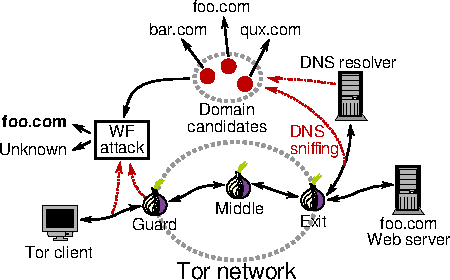
\includegraphics[width=\linewidth]{figures/attack-scenario.pdf}
	\caption{An overview of our correlation attack.  Ingress traffic is
	monitored either by a network-level adversary or the guard relay.  Egress
	traffic is monitored either by a network-level adversary or a DNS server.
	Captured DNS queries then serve as the candidate set for a Website
	fingerprinting attack.}
	\label{fig:attack-scenario}
\end{figure}

\begin{description}
	\item[Ingress sniffing] An attacker must observe traffic that is entering
		the Tor network.  The attacker can operate on the network level, i.e.,
		be a malicious ISP, or an intelligence agency.  In addition, the
		attacker can operate on the relay level, i.e., run a malicious Tor guard
		relay.  Note that in both cases, the attacker can only observe encrypted
		data.  Therefore, packet meta information such as packet lengths and
		directions serve as input to a website fingerprinting
		attack~\cite{Panchenko2016a}.
	\item[Egress sniffing] To observe both ends of the communication, an
		attacker must also observe egress DNS traffic.  We expect the adversary
		to operate on the network level, i.e., be on the path between exit relay
		and a DNS server.  Alternatively, the attacker can run a malicious DNS
		resolver or server.  Note that an attacker may also run an exit relay,
		but in that case she might as well do classical end-to-end correlation.
	\item[WF fingerprinting] We employ a website fingerprinting attack to
		determine if any of the recently observed DNS queries in egress traffic
		could be part of the encrypted ingress traffic.  Note that the DNS query
		itself does not tell us what \emph{page} a user is going to.
\end{description}

\subsection{Egress sniffing}

How many DNS requests does an exit relay see in $n$ minutes?
\begin{itemize}
	\item We can measure request frequency \emph{without} capturing payload.
	\item We further reduce noise by taking timestamp modulo $m$.
	\item We can do this on an exit relay, or on the DNS root.
	\item \texttt{tshark -f 'udp port 53' -T fields -e frame.time\_epoch -Y 'dns.qry.type == 1 and dns.flags.response == 0'}
	\item Number of requests probably depends on current bandwidth load (which
		we can obtain from the consensus) and the exit policy (which we can
		obtain from the descriptor).
	\item We can limit our exit policy to 80 and 443, so we have a decent
		baseline for requests caused by web traffic.
	\item Fetch relayed traffic from descriptors and use it to normalise
		observed DNS requests.
\end{itemize}

There are several layers of caching that we have to consider.  On the client
side:
\begin{itemize}
	\item Tor Browser has its own cache.  See the settings
		\texttt{network.dnsCache*} in \url{about:config}.
	\item The local Tor client probably (?) also has its own cache.  See the
		code in src/or/dns.c.
\end{itemize}

On the exit side:
\begin{itemize}
	\item The exit relay maintains its own caching layer around eventdns.c.  See
		the code in src/or/dns.c.
	\item The exit relay's resolver also does its own caching.
\end{itemize}

